\section{Durchführung}
\subsection{Aufbau}
\label{sec:Durchführung}
Der Aufbau besteht hauptsächlich aus einer optischen Strecke. Das Licht einer Spektrallampe wird gebündelt und auf $\lambda = \SI{794,8}{\nano \meter}$
gefiltert. Das entspricht der $\text{D}_1$ Linie von Rubidium, welches untersucht wird. Mit einer Kombination aus einem Polarisationsfilter und einer
$\sfrac{\lambda}{4}$-Platte wird das Licht rechtszirkular polarisiert. Dieses Licht durchquert eine Dampfzelle, in der eine Mischung aus die Rubidium-Isotope ${}^{87}\text{Rb}$
und ${}^{87}\text{Rb}$ gasförmig vorliegen. Die Dampfzelle ist beheizt, um einen optimalen Dampfdruck zu erzeugen. Das austretende Licht wird gebündelt
und von einem Photoelement gemessen. Die optischen Bauteile werden so justiert, dass die Intensität am Photoelement maximal ist. Die Dampfzelle ist von drei Helmholtzspulen umgeben, von denen eine zum Ausgleich des Erdmagnetfeldes sind und zwei  für
die Erzeugung der Zeeman-Niveaus. Dieser Aufbau ist in Abbildung \ref{fig:aufbaucom} skizziert.


\begin{figure}
	\centering
	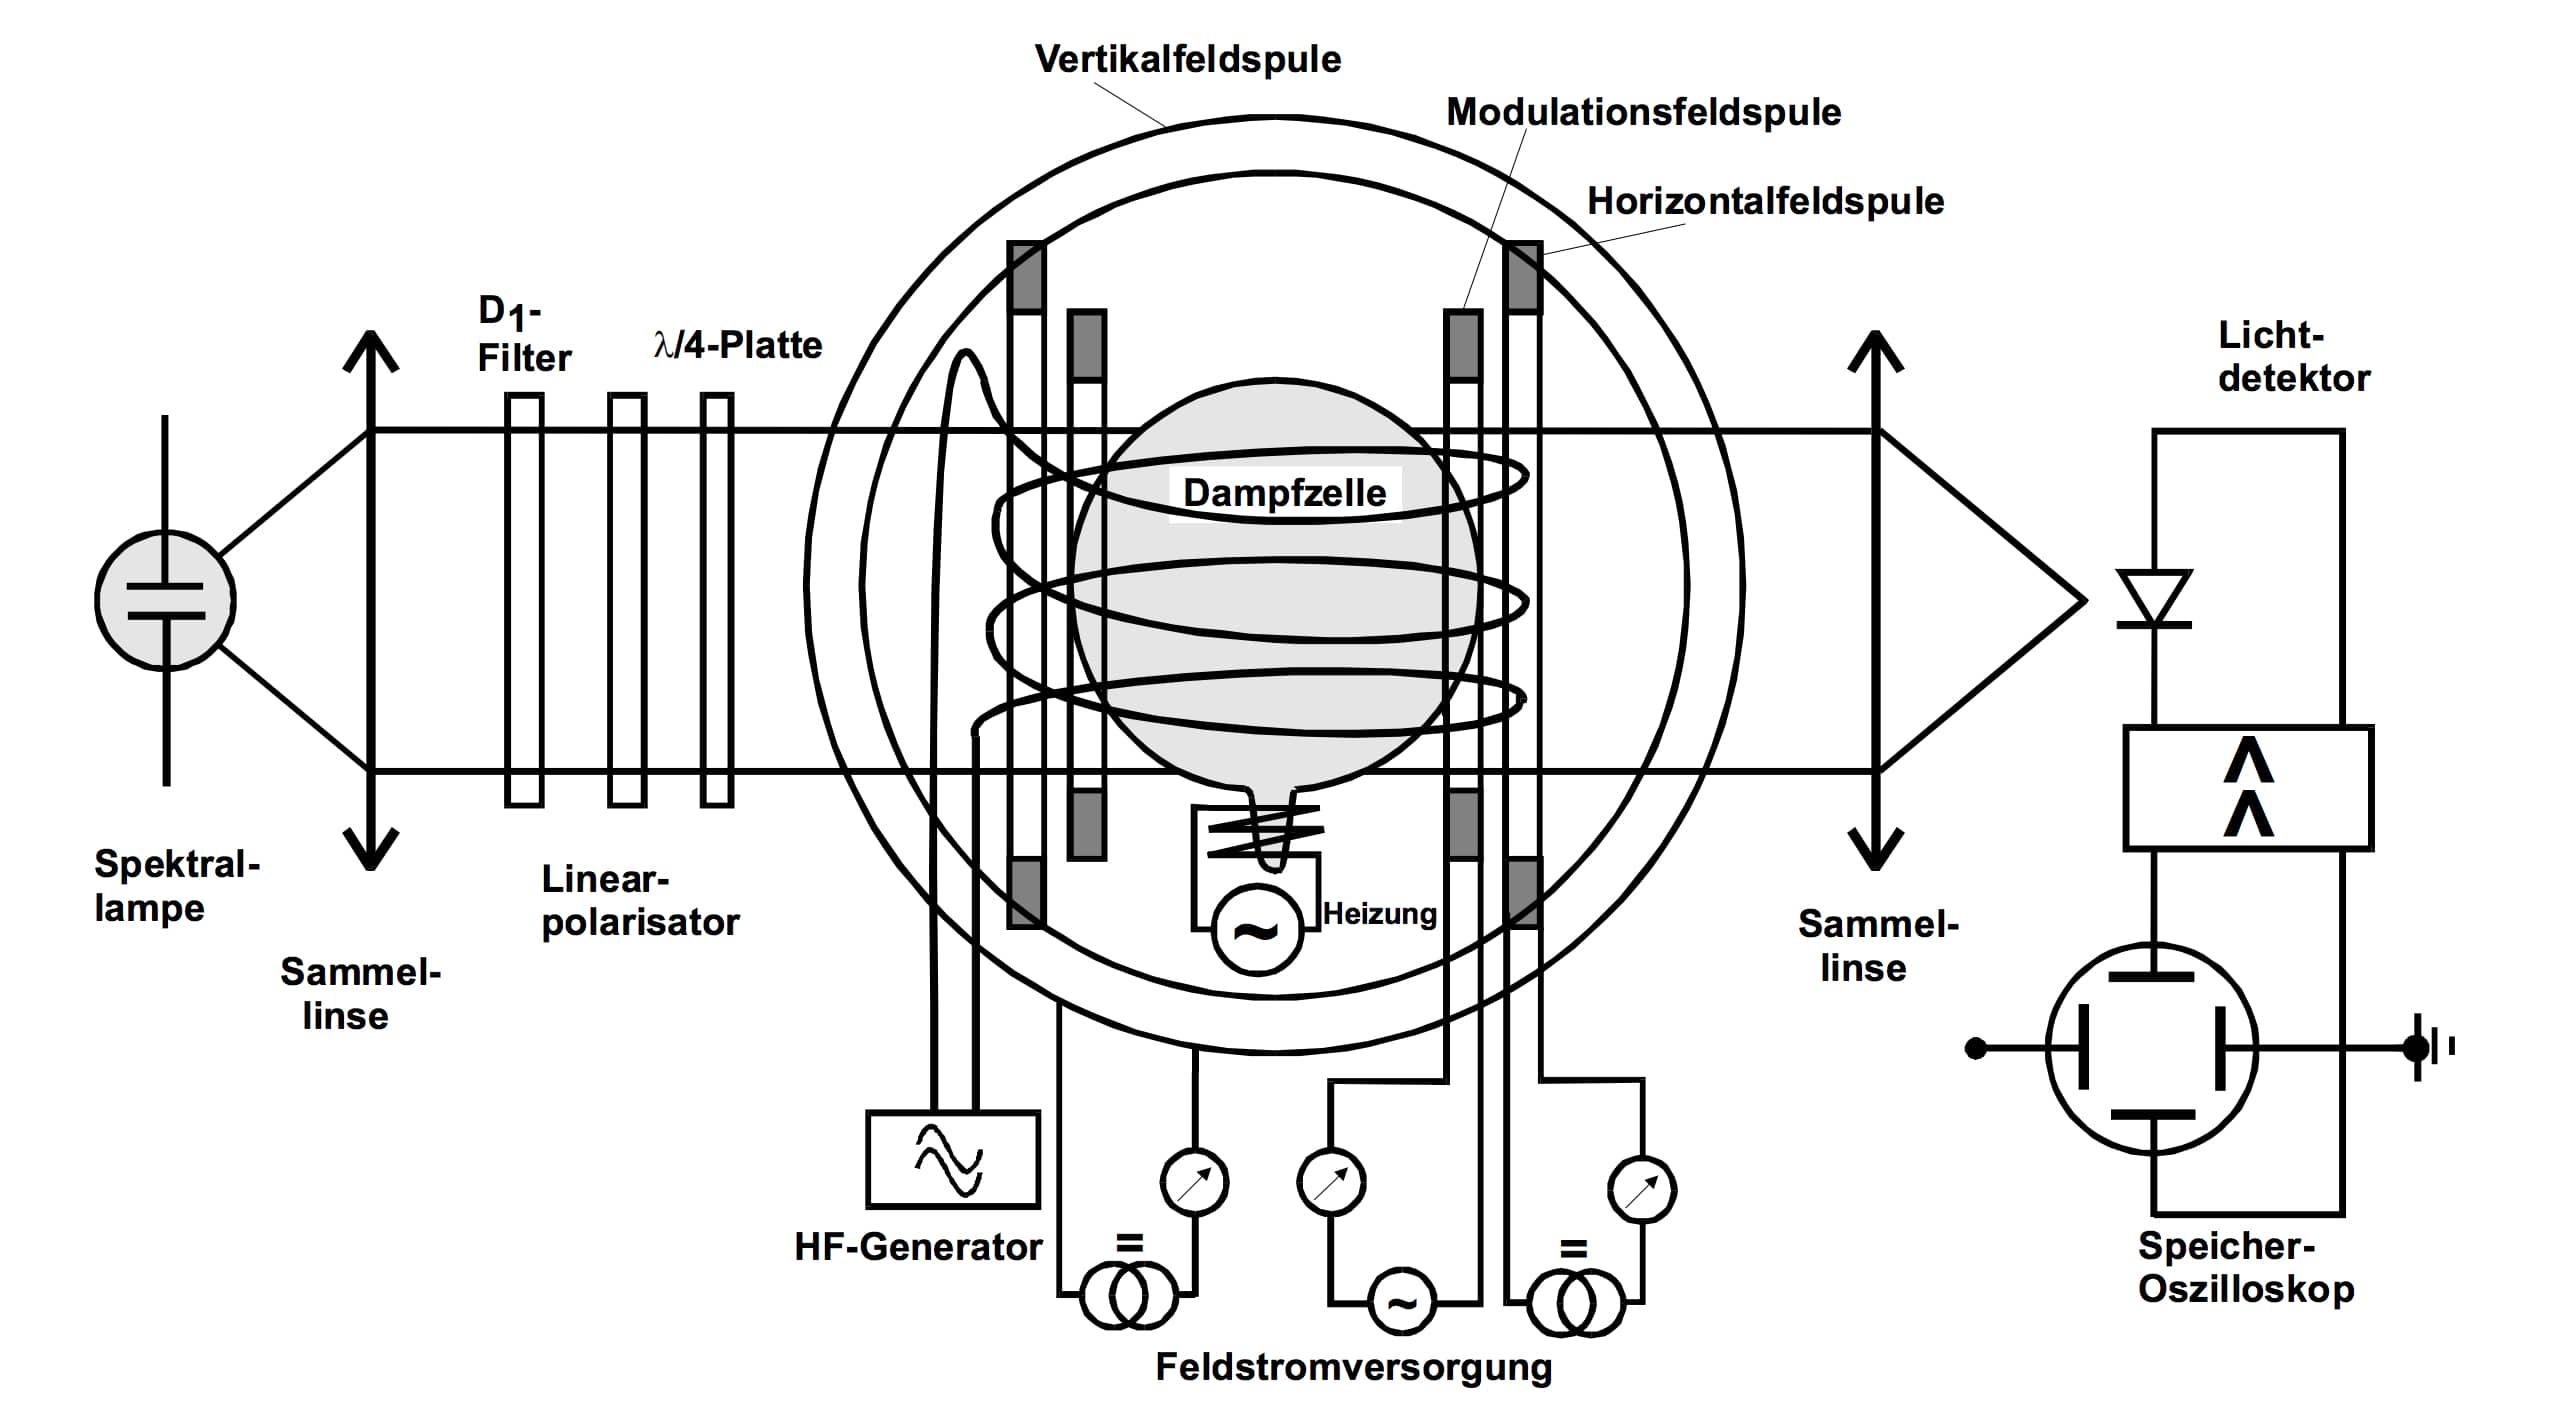
\includegraphics[width=0.8\linewidth]{img/aufbaucom.jpg}
	\caption{Schematischer Aufbau des optischen Pumpens.\cite{V21}}
	\label{fig:aufbaucom}
\end{figure}

Zunächst muss der Aufbau so gedreht werden, dass er parallel beziehungsweise antiparallel zu der Horizontalkomponente des Erdmagnetfelds steht. Als nächstes wird dessen Vertikalkomponente ausgeglichen. Dazu wird zunächst die Photodiode mit dem Kanal 2 des Oszilloskops verbunden. Auf Kanal 1 wird der Recorder-Ausgang der Sweepspule gelegt und das Oszilloskop wird auf XY Betrieb gestellt. Auf dem Oszilloskop ist nun ein breiter nach unten gerichteter Peak zu sehen. Dieser wird mithilfe der Vertikalspule auf minimale Breite gebracht. Das Nulldurchgang-Minimum entsteht durch die bei verschwindendem Magnetfeld fehlende Zeeman-Aufspaltung, wodurch kein optisches Pumpen möglich ist und die Transparenz minimal wird.

Zur Vermessung der Resonanzstelle wird die Frequenz der RF-Spule von $\SI{100}{\kilo \hertz}$ bis $\SI{1}{\mega \hertz}$ in $\SI{100}{\kilo \hertz}$-Schritten erhöht, wobei in jedem Schritt der Strom gemessen, an dem die auftretenden Resonanzstellen liegen. Zusätzlich zur Resonanzstelle bei $B = 0$ treten auch je eine Resonanzstelle für die beiden zu untersuchenden Isotope auf .... . Die Sweep-Spule wird mithilfe des Schalters Start/Reset auf Reset gestellt, wodurch ein konstantes Magnetfeld in der Apparatur vorliegt. Dabei ist der Strom, der angelegt wird, proportional zu den Umdrehungen an dem Potentiometer. Ab einer Frequenz von $\SI{200}{\kilo \hertz}$ bis $\SI{300}{\kilo \hertz}$ muss mithilfe der zusätzlichen Horizontalenspule der Sweep-Bereich auf die Resonanzstelle erweitert werden. Um das Verhältnis der Rb-Isotope zu bestimmen, wird ein Bild des Oszilloskops aufgenommen, auf dem die zwei Dips der Transparenz zu sehen sind.
